\documentclass{article}

% CS182 project report template based on the NeurIPS style.
% Keep this file short and use it as a starting point for the final report.

\usepackage[final]{neurips_2026}

\usepackage[utf8]{inputenc}
\usepackage[T1]{fontenc}
\usepackage{hyperref}
\usepackage{url}
\usepackage{booktabs}
\usepackage{amsfonts}
\usepackage{nicefrac}
\usepackage{microtype}
\usepackage{xcolor}

\usepackage{amsmath, color-edits, caption, graphicx}

\title{Mask-Guided High-Fidelity 3D Product Reconstruction via SAM2 and 3D-Consistent Gaussian Splatting Refinement}

\author{%
  Zidong Song$^{1}$\footnotemark[1] \\
  \texttt{songzd2024@shanghaitech.edu.cn}
  \and
  Boyang Zhou$^{1}$\footnotemark[1] \\
  \texttt{zhouby2024@shanghaitech.edu.cn}
  \and
  Zian Chen$^{1}$\footnotemark[1] \\
  \texttt{chenza2024@shanghaitech.edu.cn} \\
  $^{1}$ShanghaiTech University
}

\hypersetup{hidelinks}

\begin{document}

\renewcommand{\thefootnote}{\fnsymbol{footnote}}
\footnotetext[1]{Co-first authors.}

\maketitle

\begin{abstract}
Creating clean 3D object assets from casual monocular videos remains challenging due to cluttered backgrounds and reconstruction artifacts. We present MOF3R, a segmentation-guided 3D reconstruction pipeline built upon 3D Gaussian Splatting (3DGS). Object masks generated by SAM2 are used as foreground priors through a Mask-Guided Compound Loss that focuses optimization on target objects while suppressing background fitting. We further introduce a geometry-aware pruning framework that removes floating Gaussians and boundary artifacts using multi-view mask consistency, density analysis, and anisotropy constraints. Experiments on the CO3Dv2 dataset show that MOF3R produces cleaner reconstructions with fewer artifacts and sharper object boundaries than original 3DGS, demonstrating the effectiveness of combining semantic guidance with geometric refinement for object-centric 3D reconstruction.

\end{abstract}

\section{Introduction}

The acquisition of high-quality 3D digital assets is important for e-commerce, virtual reality, and the creation of digital content. Recent advances in 3D Gaussian Splatting (3DGS) have significantly improved reconstruction efficiency over Neural Radiance Fields (NeRF), enabling fast training and real-time rendering while maintaining high visual quality.

Despite these advantages, applying 3DGS to casually captured mobile videos remains challenging. Such videos often contain cluttered backgrounds, limited viewpoints, and image degradations, causing Gaussian primitives to be allocated to irrelevant regions. Consequently, reconstructions frequently suffer from floating artifacts, noisy structures, and inaccurate object boundaries, reducing asset quality and usability.

Recent progress in video object segmentation provides a promising solution through semantic foreground priors. In particular, SAM2 can generate reliable object masks in video sequences. However, existing reconstruction pipelines typically use segmentation only as a preprocessing step and do not fully exploit semantic information during optimization and geometric refinement.

To address this limitation, we propose Masked Object Fidelity 3D Reconstruction (MOF3R), an object-centric reconstruction framework for monocular videos. The foreground masks generated by SAM2 are incorporated into 3DGS optimization through a Mask-Guided Compound Loss that focuses on the surveillance of target objects and suppresses background fitting. We further introduce a geometry-aware pruning strategy based on multi-view consistency, local density analysis, and anisotropy constraints to remove floating artifacts and refine object boundaries.

The main contributions of this work are summarized as follows:

\begin{enumerate}
\item We present a segmentation-guided object-centric 3DGS reconstruction framework for generating high-quality 3D assets from casually captured videos.

\item We introduce a Mask-Guided Compound Loss that incorporates foreground semantic priors into 3DGS optimization, reducing background interference, and improving reconstruction quality.

\item We propose a geometry-aware pruning strategy that combines multi-view consistency, local geometric structure, and anisotropy analysis to remove floating artifacts while preserving fine details.

\end{enumerate}

Experiments on the CO3Dv2 data set demonstrate that the proposed method produces cleaner reconstructions and sharper object boundaries than the original 3DGS.

\section{Method}

\subsection{Overview}

Our goal is to reconstruct a high-fidelity object-centric 3D representation from a monocular video. Given an input video sequence $V={I_i}_{i=1}^{N}$, we first estimate camera parameters $C={K_i,T_i}_{i=1}^{N}$ using COLMAP and obtain foreground masks $M={M_i}_{i=1}^{N}$ with SAM2.

Building upon these semantic priors, we propose a reconstruction framework that combines mask-guided optimization with geometry-aware refinement. During training, foreground masks are incorporated into the 3D Gaussian Splatting (3DGS) optimization process to suppress background fitting. After reconstruction, we apply a multi-metric pruning strategy based on multi-view consistency and local geometric properties to remove floating artifacts and refine object boundaries. The overall pipeline is illustrated in Figure~\ref{fig:schematic}.

\begin{figure}[t]
    \centering
    \includegraphics[width=1\linewidth]{pics/MOF3R_overview.png}
    \caption{MOF3R: Overall pipeline schematic}
    \label{fig:schematic}
\end{figure}

\subsection{Mask-Guided Optimization}

A major challenge of object-centric reconstruction from unconstrained videos is that standard 3DGS optimizes all image pixels equally, causing Gaussian primitives to fit both the target object and surrounding background regions.

To focus optimization on the object of interest, we incorporate foreground masks generated by SAM2 into the training objective. Given a ground-truth image $I$, rendered image $\hat I$, and binary mask $M$, we define a mask-constrained L1 loss as

$$
\mathcal{L}_{L1}^{mask} = |M\odot(I-\hat I)|_1
$$

where $\odot$ denotes multiplication by element. This formulation restricts photometric supervision to foreground regions and suppresses background fitting during the early stages of optimization.

Directly applying structural similarity loss only inside the mask may introduce instability near object boundaries. Therefore, we construct a composite image

$$
I_{comp} = M\odot\hat I + (1-M)\odot I
$$

where rendered foreground pixels are blended with the original background. The SSIM loss is then computed on the composite image:

$$
\mathcal{L}_{\mathrm{SSIM}}^{mask} = 1-\mathrm{SSIM}(I, I_{comp})
$$

The final training objective is defined as

$$
\mathcal{L} = \lambda_1\mathcal{L}_{L1}^{mask} + \lambda_2\mathcal{L}_{\mathrm{SSIM}}^{mask}
$$

This compound objective encourages Gaussian primitives to concentrate on the target object while preserving global image consistency, resulting in cleaner reconstructions and fewer background artifacts.

\subsection{Geometry-Aware Multi-Metric Pruning}

Although mask-guided optimization effectively suppresses most background interference, the reconstructed model may still contain floating Gaussians and elongated boundary artifacts caused by limited viewpoints and optimization errors. To further improve reconstruction quality, we introduce a geometry-aware multi-metric pruning strategy.

\subsubsection{Multi-view Mask Consistency} 

For each Gaussian center $g_j$, we project its 3D position into all visible camera views and examine whether the projected point lies within the corresponding foreground masks.

Gaussians that consistently fall outside foreground regions across multiple valid views are considered background artifacts and removed. To avoid incorrect pruning caused by occlusions, only visible views participate in the voting process.

This consistency check effectively eliminates isolated floating Gaussians around the reconstructed object.

\subsubsection{Density and Anisotropy Filtering}

Multi-view consistency alone is insufficient to remove all boundary artifacts. Therefore, we further analyze the local geometric structure of each Gaussian using a K-nearest-neighbor (KNN) neighborhood.

For each Gaussian primitive, we estimate its local density and anisotropy level from neighboring Gaussians. A Gaussian is marked as an outlier if it simultaneously exhibits:

\begin{enumerate}
    \item significantly lower local density than its neighborhood;
    \item excessive anisotropy beyond a predefined threshold.
\end{enumerate}

Such primitives typically correspond to stretched structures and trailing artifacts near object boundaries. Removing them leads to a cleaner and more compact reconstruction.

\subsubsection{Adaptive Shrinkage}

Directly removing all boundary candidates may damage fine structures. To preserve delicate geometric details, we introduce an adaptive shrinkage mechanism.

Instead of immediately deleting uncertain boundary Gaussians, we gradually reduce their scale and opacity:

$$
s'=\alpha s,\qquad
o'=\beta o
$$

where $0<\alpha,\beta<1$.

This progressive refinement smooths object boundaries while retaining high-confidence geometric structures, resulting in a cleaner and visually sharper reconstruction.

\section{Experiments}

\subsection{Experimental Setup}

We evaluate our method on the CO3Dv2 dataset, a large-scale benchmark containing multi-view video captures of real-world objects under diverse viewpoints and backgrounds. To stress-test reconstruction quality in challenging scenarios, we focus on categories such as Bowl and Teddy, which contain thin-walled structures, self-occlusions, and complex geometries.

\subsection{Preprocessing}

For each video sequence, frames are extracted at a fixed frame rate and camera intrinsics/extrinsics are estimated using COLMAP. Foreground object masks are generated with SAM2 using a single user-provided prompt on the first frame.

\subsection{Training Details}

We build our method on top of the original 3D Gaussian Splatting (3DGS) framework. During optimization, we apply the proposed Mask-Guided Compound Loss, which combines mask-constrained L1 supervision with a composite-image SSIM loss. The loss weights $\lambda_1$ and $\lambda_2$ are empirically set to balance photometric accuracy and structural consistency.

After reconstruction, we apply the proposed Geometry-Aware Multi-Metric Pruning procedure, including multi-view mask consistency checking, KNN-based density and anisotropy filtering, and adaptive shrinkage refinement.

\subsection{Baseline and Metrics}

We compare our method against original 3D Gaussian Splatting (3DGS) trained directly on the original video frames without segmentation guidance.

We report the following metrics to evaluate reconstruction quality:

\begin{itemize}
    \item PSNR (Peak Signal-to-Noise Ratio)
    \item SSIM (Structural Similarity Index)
    \item LPIPS (Learned Perceptual Image Patch Similarity)
\end{itemize}

In addition, we provide qualitative comparisons focusing on background suppression, boundary sharpness, and the removal of floating artifacts.

\subsection{Quantitative Results}

Table~\ref{tab:main} reports quantitative results on representative CO3Dv2 sequences.

\begin{table}[t]
\centering
\caption{Quantitative comparison on CO3Dv2 sequences.
Metrics are evaluated within foreground mask regions.}
\label{tab:main}
\begin{tabular}{lccc}
\toprule
Method & PSNR$\uparrow$ & SSIM$\uparrow$ & LPIPS$\downarrow$\\
\midrule
Original 3DGS & 19.07 & 0.592 & 0.629 \\
Mask-Guided & 21.03 & 0.931 & 0.125 \\
MOF3R (ours) & \textbf{23.56} & \textbf{0.935} & \textbf{0.120} \\
\bottomrule
\end{tabular}
\end{table}

Figure~\ref{fig:result} visualizes the quantitative performance in different object sequences. The proposed pipeline consistently improves perceptual quality while maintaining
high structural similarity.

\begin{figure}
    \centering
    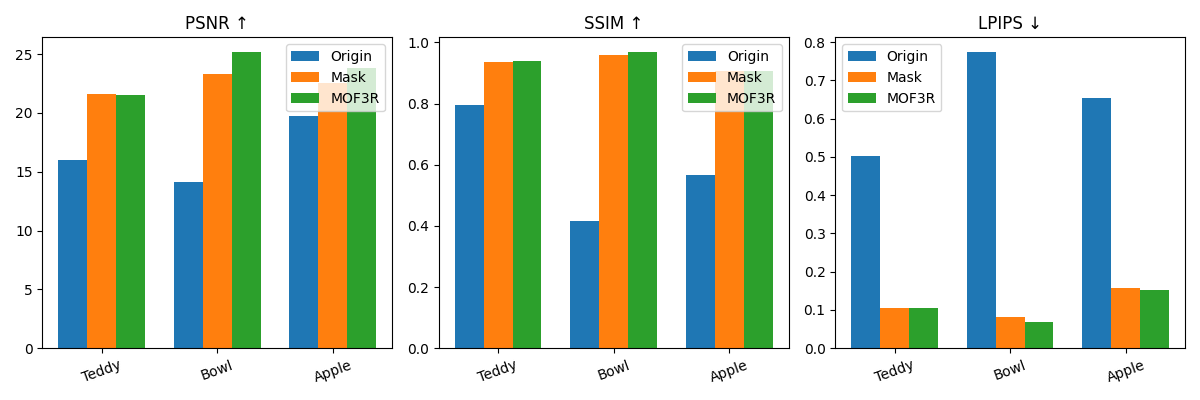
\includegraphics[width=\linewidth]{pics/result.png}
    \caption{Comparison of reconstruction quality across representative
CO3Dv2 sequences.}
    \label{fig:result}
\end{figure}

Compared with original 3DGS, our full pipeline improves the average PSNR from 19.07 dB to 23.56 dB and reduces LPIPS from 0.629 to 0.120. These improvements indicate that semantic guidance effectively suppresses background fitting while geometric pruning removes residual artifacts.

The proposed geometry-aware pruning stage further improves reconstruction quality by removing residual floating artifacts and elongated Gaussian primitives. The improvements are particularly evident on challenging objects such as Bowl, where the full pipeline improves PSNR from 14.10 dB to 25.17 dB while reducing LPIPS from 0.774 to 0.068.

Full per-sequence quantitative results, including different pruning configurations and training iterations, are provided in Appendix~\ref{sec:full_result}.

\subsection{Qualitative Results}

Figure~\ref{fig:qualitative} presents qualitative
comparisons on representative CO3Dv2 scenes. Qualitative comparisons further demonstrate cleaner object boundaries, fewer background artifacts, and more compact Gaussian distributions, validating the complementary benefits of semantic guidance and geometric refinement.

Without foreground supervision, original 3DGS tends to allocate Gaussian primitives to background regions, resulting in severe floating artifacts and blurred object boundaries.

By introducing the proposed mask-guided loss, the optimization process becomes object-centric and substantially suppresses background interference. However, a small number of residual artifacts remain around object boundaries.

The proposed geometry-aware pruning stage further removes isolated and elongated Gaussian primitives, producing cleaner silhouettes and more compact reconstructions. The improvement is particularly visible on the TeddyBear, Bowl, and Apple scenes, where boundary sharpness and visual consistency are significantly enhanced.

\begin{figure*}[t]
    \centering
    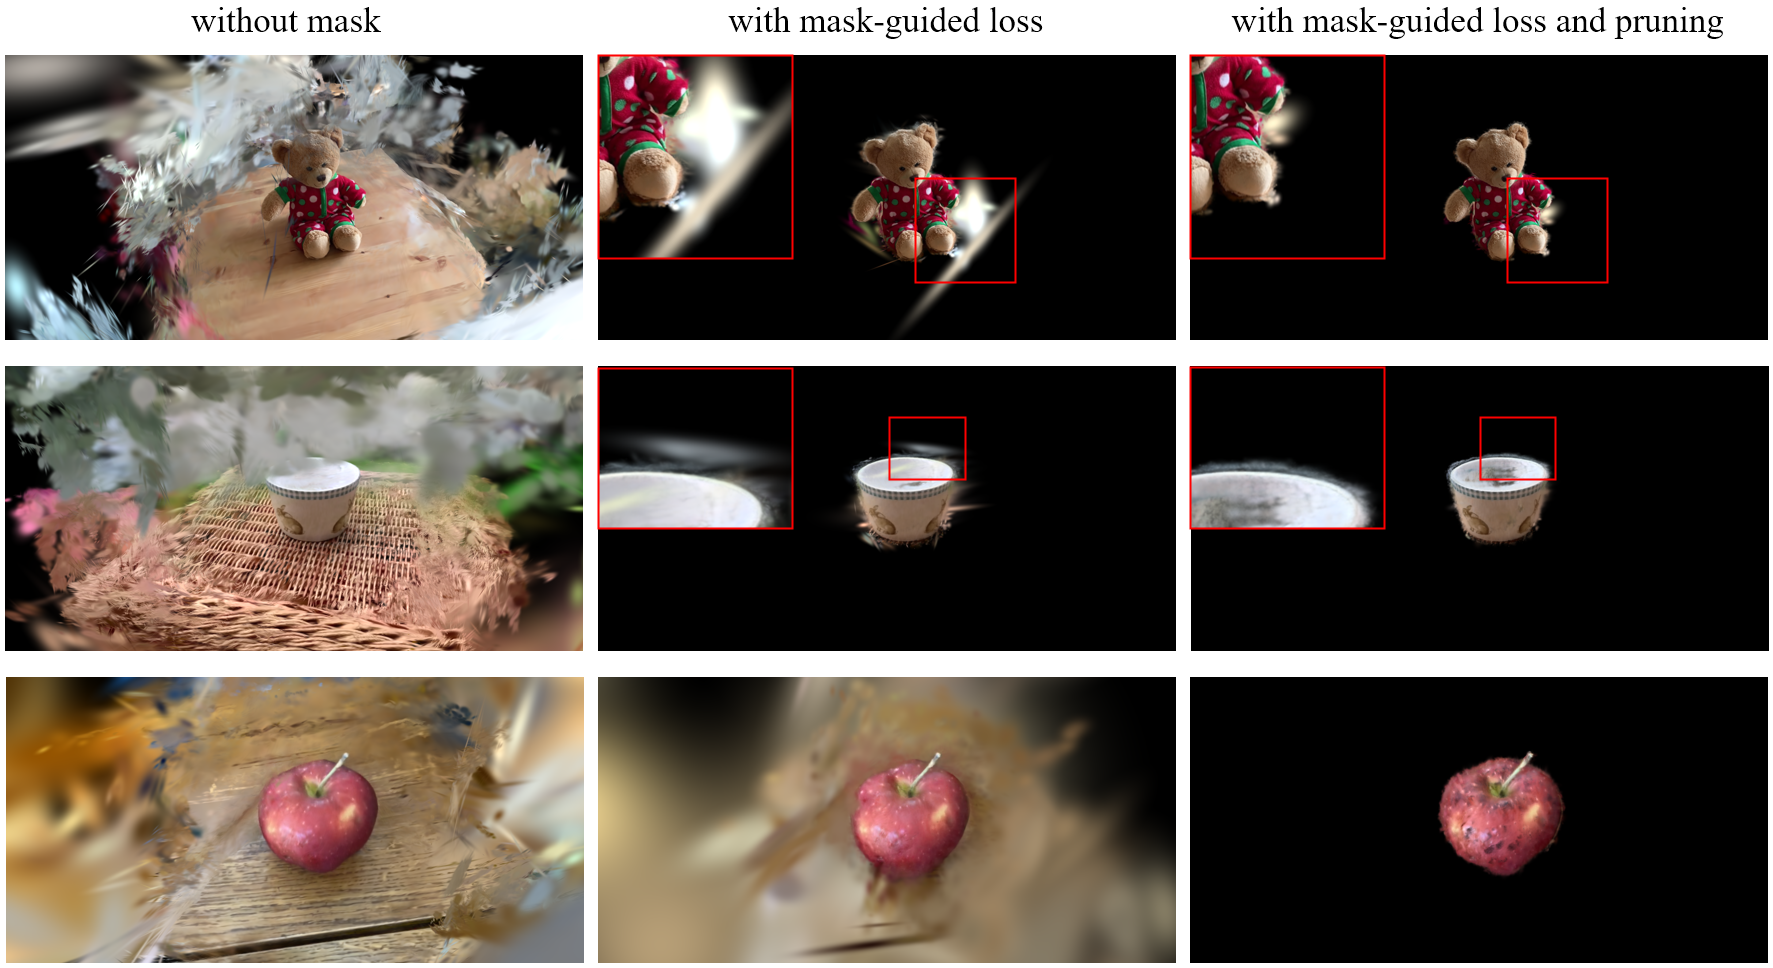
\includegraphics[width=\textwidth]{pics/comparsion.png}
    \caption{
    Qualitative comparison of reconstruction results.
    From left to right: original 3DGS, reconstruction with the proposed mask-guided loss, and the full MOF3R pipeline with geometry-aware pruning.
    The mask-guided loss effectively suppresses background interference, while the pruning stage further removes floating artifacts and improves object boundary quality.
    }
    \label{fig:qualitative}
\end{figure*}

\subsection{Ablation Study}

We conduct an ablation study to evaluate the contribution of each component in the proposed pipeline.

Starting from original 3DGS, we first introduce the mask-guided compound loss, which restricts optimization to foreground regions. We then apply the proposed geometry-aware pruning strategy to remove residual artifacts and elongated Gaussian primitives.

Results in Table~\ref{tab:ablation} show that the pruning stage further improves reconstruction quality by removing floating artifacts and refining object boundaries where Reasonable pruning showcases the best performance.

\begin{table}[t]
\centering
\caption{Effect of different pruning strategies.}
\label{tab:ablation}
\begin{tabular}{lccc}
\toprule
Pruning Type & PSNR$\uparrow$ & SSIM$\uparrow$ & LPIPS$\downarrow$\\
\midrule
None & 21.03 & 0.931 & 0.125\\
Conservative & 23.18 & 0.933 & 0.123\\
Reasonable & \textbf{23.56} & \textbf{0.935} & \textbf{0.120}\\
Aggressive & 23.42 & 0.932 & 0.121\\
\bottomrule
\end{tabular}
\end{table}


\section{Conclusion}

% 这个现在是 AI 写的，一定要找时间人工审核一下！！！

In this work, we presented MOF3R, a segmentation-guided framework for object-centric 3D reconstruction from monocular videos. By incorporating SAM2-generated foreground masks into the 3D Gaussian Splatting optimization process, our Mask-Guided Compound Loss encourages Gaussian primitives to focus on the target object while suppressing background fitting. We further introduced a geometry-aware multi-metric pruning strategy that combines multi-view mask consistency, local density analysis, and anisotropy filtering to remove floating artifacts and refine object boundaries.

Experiments on challenging categories from the CO3Dv2 dataset demonstrate that the proposed approach produces cleaner reconstructions with fewer background artifacts and sharper object boundaries compared with original 3DGS. The results suggest that semantic priors and geometric refinement provide complementary benefits for object-centric reconstruction in unconstrained environments.

For future work, we plan to investigate tighter integration between segmentation and reconstruction, as well as more robust geometric regularization techniques for handling transparent objects, reflective surfaces, and highly occluded scenes.

\nocite{*}
\bibliographystyle{unsrtnat}
\bibliography{ref}

\newpage
\appendix

\section{Full Quantitative Results}
\label{sec:full_result}

This appendix provides the complete quantitative results
for all evaluated sequences, training iterations, and
pruning configurations.

\begin{table}[h!]
    \centering
    \begin{tabular}{c|c|c|c|c|c} \toprule
group & scene id & iteration lable & psnr-mean & ssim-mean & lpips-mean \\ \midrule
origin & teddy & 1000 & 15.957719 & 0.795733 & 0.502974 \\
origin & teddy & 3000 & 18.866552 & 0.833170 & 0.392285 \\
origin & bowl & 1000 & 14.101571 & 0.415512 & 0.773754 \\
origin & bowl & 3000 & 16.563001 & 0.589804 & 0.452322 \\
origin & apple & 1000 & 19.714700 & 0.566154 & 0.653520 \\
origin & apple & 3000 & 26.401725 & 0.809528 & 0.210779 \\
mask & teddy & 1000 & 15.014329 & 0.844903 & 0.262621 \\
mask & teddy & 3000 & 21.628734 & 0.937388 & 0.105317 \\
mask & bowl & 1000 & 19.890134 & 0.929169 & 0.127335 \\
mask & bowl & 3000 & 23.286411 & 0.959550 & 0.082352 \\
mask & apple & 1000 & 16.627887 & 0.781926 & 0.312548 \\
mask & apple & 3000 & 22.528242 & 0.905894 & 0.157318 \\
MOF3R & teddy & 1000 & 12.385004 & 0.743488 & 0.426430 \\
MOF3R & teddy & 1000-mask-pruned & 12.493246 & 0.746858 & 0.422140 \\
MOF3R & teddy & 1000-mask-pruned-aggressive & 12.659274 & 0.746094 & 0.416255 \\
MOF3R & teddy & 1000-mask-pruned-conservative & 12.586952 & 0.745608 & 0.422369 \\
MOF3R & teddy & 1000-mask-pruned-extreme & 12.659274 & 0.746094 & 0.416255 \\
MOF3R & teddy & 1000-mask-pruned-reasonable & 12.654369 & 0.747885 & 0.416781 \\
MOF3R & teddy & 3000 & 19.715921 & 0.921837 & 0.153458 \\
MOF3R & teddy & 3000-mask-pruned & 20.170774 & 0.924714 & 0.149210 \\
MOF3R & teddy & 3000-mask-pruned-aggressive & 21.969686 & 0.927167 & 0.137814 \\
MOF3R & teddy & 3000-mask-pruned-conservative & 21.317001 & 0.929250 & 0.140480 \\
MOF3R & teddy & 3000-mask-pruned-extreme & 21.969686 & 0.927167 & 0.137814 \\
MOF3R & teddy & 3000-mask-pruned-reasonable & 21.715209 & 0.930042 & 0.137910 \\
MOF3R & bowl & 1000 & 20.116411 & 0.931011 & 0.126487 \\
MOF3R & bowl & 1000-mask-pruned & 20.264461 & 0.933845 & 0.122918 \\
MOF3R & bowl & 1000-mask-pruned-aggressive & 22.358688 & 0.953486 & 0.091790 \\
MOF3R & bowl & 1000-mask-pruned-conservative & 21.520443 & 0.946677 & 0.103117 \\
MOF3R & bowl & 1000-mask-pruned-extreme & 22.358688 & 0.953486 & 0.091790 \\
MOF3R & bowl & 1000-mask-pruned-reasonable & 21.783171 & 0.948651 & 0.099945 \\
MOF3R & bowl & 3000 & 23.339291 & 0.959306 & 0.082510 \\
MOF3R & bowl & 3000-mask-pruned & 23.688310 & 0.961111 & 0.079778 \\
MOF3R & bowl & 3000-mask-pruned-aggressive & 25.359025 & 0.967092 & 0.068848 \\
MOF3R & bowl & 3000-mask-pruned-conservative & 24.791282 & 0.966737 & 0.070560 \\
MOF3R & bowl & 3000-mask-pruned-extreme & 25.359025 & 0.967092 & 0.068848 \\
MOF3R & bowl & 3000-mask-pruned-reasonable & 25.170994 & 0.967742 & 0.068185 \\
MOF3R & apple & 1000 & 16.801979 & 0.786755 & 0.300191 \\
MOF3R & apple & 1000-mask-pruned & 17.028800 & 0.794986 & 0.294224 \\
MOF3R & apple & 1000-mask-pruned-aggressive & 17.036958 & 0.774801 & 0.316318 \\
MOF3R & apple & 1000-mask-pruned-conservative & 17.145694 & 0.791379 & 0.299683 \\
MOF3R & apple & 1000-mask-pruned-extreme & 17.036958 & 0.774801 & 0.316318 \\
MOF3R & apple & 1000-mask-pruned-reasonable & 17.171169 & 0.785992 & 0.306671 \\
MOF3R & apple & 3000 & 22.499137 & 0.905678 & 0.157529 \\
MOF3R & apple & 3000-mask-pruned & 22.727309 & 0.907408 & 0.155726 \\
MOF3R & apple & 3000-mask-pruned-aggressive & 23.708253 & 0.900295 & 0.156291 \\
MOF3R & apple & 3000-mask-pruned-conservative & 23.429492 & 0.906389 & 0.156643 \\
MOF3R & apple & 3000-mask-pruned-extreme & 23.708253 & 0.900295 & 0.156291 \\
MOF3R & apple & 3000-mask-pruned-reasonable & 23.783064 & 0.906305 & 0.153110 \\ \bottomrule
    \end{tabular}
    \caption{The Result of all Metrics.}
    \label{tab:all_result}
\end{table}

\paragraph{Iteration Label Definition.}
The \textit{iteration label} column indicates the reconstruction
stage at which the evaluation was performed:

\begin{itemize}
    \item \textbf{1000}, \textbf{3000}: reconstruction results obtained after 1,000 and 3,000 optimization iterations, respectively.
    
    \item \textbf{1000-mask-pruned}, \textbf{3000-mask-pruned}: results after applying the proposed geometry-aware pruning procedure to the corresponding reconstruction checkpoint.
    
    \item \textbf{1000-mask-pruned-conservative}: pruning using relatively loose thresholds to preserve more Gaussian primitives and fine structures.
    
    \item \textbf{1000-mask-pruned-reasonable}: the default pruning configuration used in our final pipeline, balancing artifact removal and structure preservation.
    
    \item \textbf{1000-mask-pruned-aggressive}: pruning using stricter thresholds to remove a larger number of potentially noisy Gaussian primitives.
    
    \item \textbf{1000-mask-pruned-extreme}: an even more aggressive pruning configuration designed to investigate the upper limit of artifact removal.
\end{itemize}

The same naming convention applies to the corresponding
3,000-iteration checkpoints.

\end{document}
